\chapter{Experiment 1}

\epigraph{\textit{On est trop souvent imprécis lorsqu'on fait une citation.}}{Quelqu'un, un jour.}

Full 1st experiment explanation

\section{General}

\subsection{Code}
\begin{lstlisting}
print("Launch!")
qc.h(init_q)
for w in range(max_shots):
    for i in range(shots):
        qc.rx(-pi/(shots-i), init_q)
        qc.rz(pi/(shots/8), init_q)
        #qc.u(pi/(shots-i), pi/(shots/8), 0, init_q)
        z, z_north, z_south = complex_cal(qc, statevector_sim)
        if z != 0:
            if z_north != 0:
                tab_temp[0].append(z)
                tab_temp[1].append(z_north)
            if z_south != 0:
                tab_temp[0].append(z)
                tab_temp[2].append(z_south)
    qc.barrier()
    
    if (w + 1) % 5 == 0:
        print("Full circuit bloch :", w+1, "/", max_shots)

print("Fini!")
\end{lstlisting}

\subsection{Run 1 full circuit block only}

\subsection{Run 10 full circuit block only}

\subsection{Run 100 full circuit block only}

\begin{figure}[ht!]
        \centering
        \begin{subfigure}[c]{0.5\textwidth}
                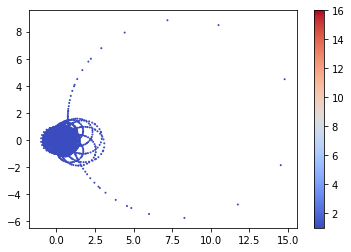
\includegraphics[width=\textwidth]{Chapitre1/Figures/exp1_100_nonZoom.png}
                \caption{Graph from 10000 data statevector without zoom}
        \end{subfigure}%
        \begin{subfigure}[c]{0.5\textwidth}
                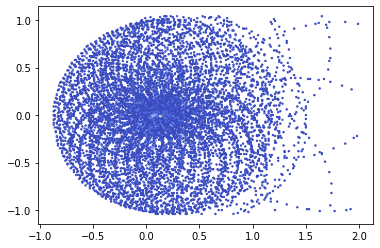
\includegraphics[width=\textwidth]{Chapitre1/Figures/exp1_100_zoom.png}
                \caption{Graph with zoom of [[-1:2][-1:1]]}
        \end{subfigure}
        \caption{Resulting of 10000 data statevector}
\end{figure}




